\section{Filtrace}

Filtrace vstupního signálu probíhala pomocí funkce "signal.sosfilt" stejně jako u odezvy na jednotkový impuls a to tak, že se postupně na vstupní signál spustil každý navrhnutý filtr.
Následně byli vytvořeny spektrogramy a grafy spektrální hustoty pro kontrolu, že se opravdu povedlo rušivé frekvence vyfiltrovat a následně byl tento vyfiltrovaný signál uložen.

\subsection{Elliptic filtry}
\begin{figure}[H] 
	\centering
	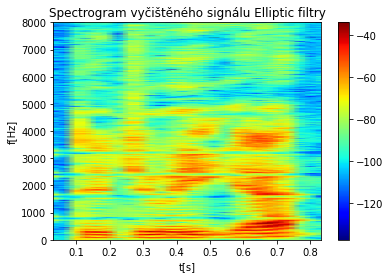
\includegraphics[scale=0.65,keepaspectratio]{Figure_20}
	\caption{Výkonový spektrogram vyčištěného signálu Elliptic filtry}
\end{figure}

\begin{figure}[H] 
	\centering
	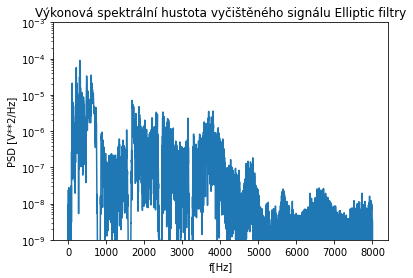
\includegraphics[scale=0.65,keepaspectratio]{Figure_21}
	\caption{Výkonová spektrální hustota vyčištěného signálu Elliptic filtry}
\end{figure}

\begin{landscape}
\begin{figure}[H] 
	\centering
	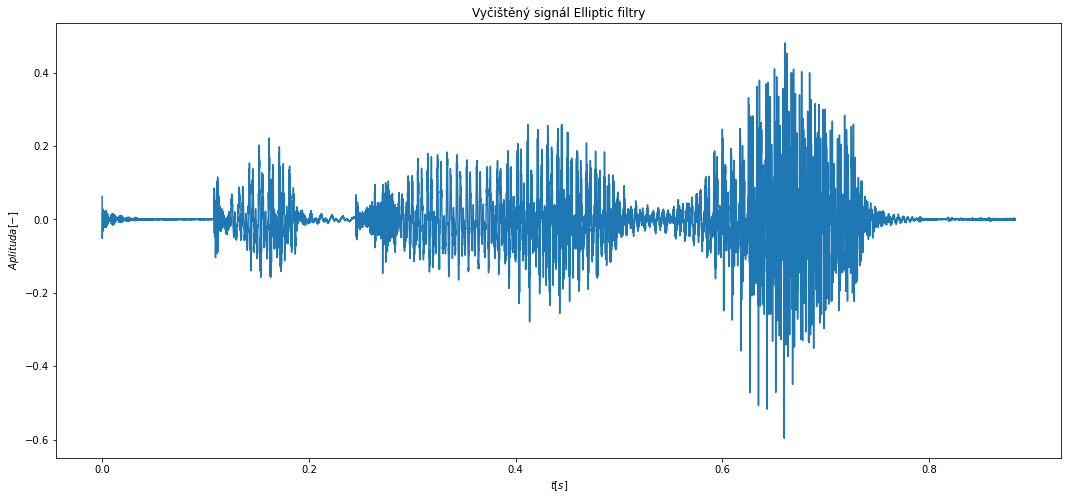
\includegraphics[scale=0.5,keepaspectratio]{Figure_23}
	\caption{Výsledný vyčištěný signál Elliptic filtry}
\end{figure}
\end{landscape}

\subsection{Butterworth filtry}
\begin{figure}[H] 
	\centering
	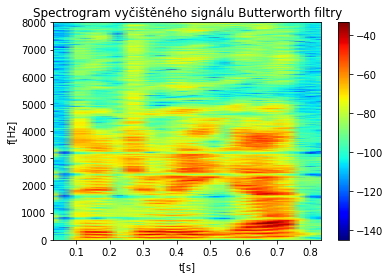
\includegraphics[scale=0.65,keepaspectratio]{Figure_27}
	\caption{Výkonový spektrogram vyčištěného signálu Butterworth filtry}
\end{figure}

\begin{figure}[H] 
	\centering
	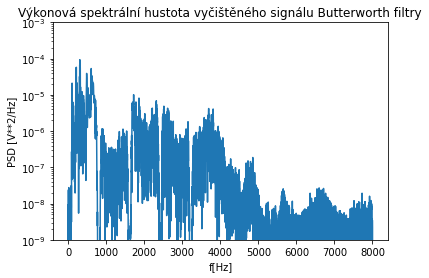
\includegraphics[scale=0.65,keepaspectratio]{Figure_28}
	\caption{Výkonová spektrální hustota vyčištěného signálu Butterworth filtry}
\end{figure}

\begin{landscape}
\begin{figure}[H] 
	\centering
	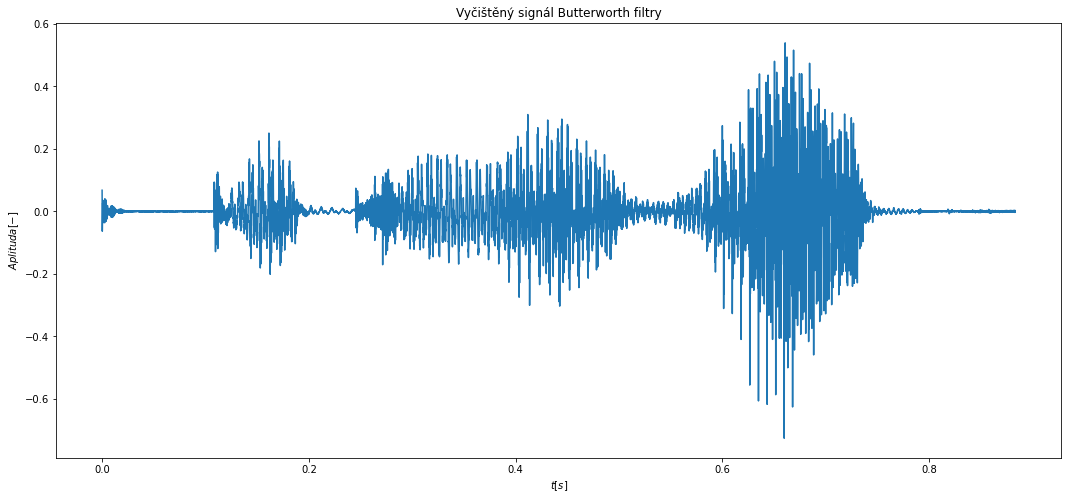
\includegraphics[scale=0.5,keepaspectratio]{Figure_29}
	\caption{Výsledný vyčištěný signál Butterworth filtry}
\end{figure}
\end{landscape}

\subsection{Shrnutí filtrace}
Vzhledem k tomu že se Butterworth filtr choval lépe ve frekvenční charakteristice tak byl použit ten na finální filtrování.